%!TEX root = Qualificacao.tex

\begin{exmp}[RaCSS applied to a 2nd order linear system] \label{ex:52}

In this example, the same cases contemplated in the previous example are considered, but with the following modifications:
\begin{enumerate}
   \setlength\itemsep{0.1pt}
   \item The index used to calculate the RIPs \eqref{eq:Jcal}, is formed according to \eqref{eq:Jracss}, i.e., the RaCSS procedure is used, described in Section \ref{sec:CSS_metod}, now taking into account the tracking error information in the RIPs updating procedure.
    \item Several simulations, or realizations, are analyzed, but maintaining the same training data, i.e. $\tilde{\bm{u}}$ and $\tilde{\bm{y}}$ remain the same for each realization. What changes are the candidate models chosen during the procedure, since this choice is based on a Bernoulli process.
\end{enumerate}

As a first step, the evolution of RIPs are analyzed for 5 different values of $\alpha$, which are: $\alpha=0$, $\alpha=0.25$, $\alpha=0.5$, $\alpha=0.75$, $\alpha=1$.

% \begin{description}
   % \setlength\itemsep{0.1pt}
  % \item[caso 1] $\alpha =0$, i.e, $J=J_s$;
  % \item[caso 2] $\alpha = 0.25$, i.e. $J=0.25J_s+0.75J_p$;
  % \item[caso 3] $\alpha = 0.5$, i.e. $J=0.5J_s+0.5J_p$;
  % \item[caso 4] $\alpha = 0.75$, i.e. $J=0.75J_s+0.25J_p$;
  % \item[caso 5] $\alpha = 1$, i.e, $J=J_r$.
% \end{description}
%
The 5 cases, considering that there is no measurement noise and with the same values as Example \ref{ex:sis2aord}, are analyzed for the RaCSS procedure. The evolution of the RIPs for each case is presented by Figure \ref{fig:exp51_ev_rips_a1_SR}.
  \begin{figure}[htpb]
    \centering
    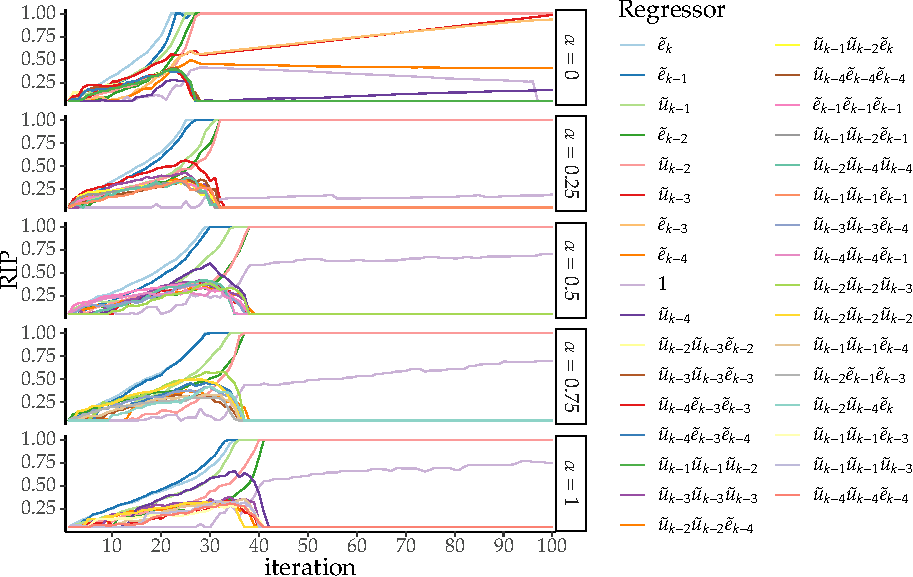
\includegraphics{Figs/Cap5/ex51_rips_evol_SR.tex.pdf}
    \caption{RIPs evolution to different values of parameter $\alpha$ considering data without noise.}
    \label{fig:exp51_ev_rips_a1_SR}
  \end{figure}
It is observed that when increasing the value of $\alpha$, regressors that do not belong to the set of ideal regressors are less frequently selected, when compared to the case where no closed loop information is used (case with $\alpha=0$) \footnote { note that the case where $\alpha=0$ in this example corresponds to case A of Example \ref{ex:sis2aord}.}.

Note that, for this realization, for $\alpha=0.5$ and $\alpha=1$ the algorithm was interrupted around iterations 60 and 90, respectively, due to the stop criterion \eqref{eq:crit.par} having been satisfied. It is emphasized that this occurs for this specific realization, the same may not happen for other realizations, due to the random character of the method.
Despite this, in general, when performing several iterations, it is possible to notice that the general behavior of Figure \ref{fig:exp51_ev_rips_a1_SR} prevails, with greater choices of spurious RIPs for the case, in which $\alpha=0$, when compared to the others ($\alpha>0$).

To analyze the behavior more generally, 50 realizations are made (with the same training data) for each value of $\alpha$. The density of probability of convergence of the RIPs for each value of $\alpha$, as a function of the number of iterations, is shown in Figure \ref{fig:exp51_dens_prob_SR}.
\begin{figure}[htpb]
  \centering
  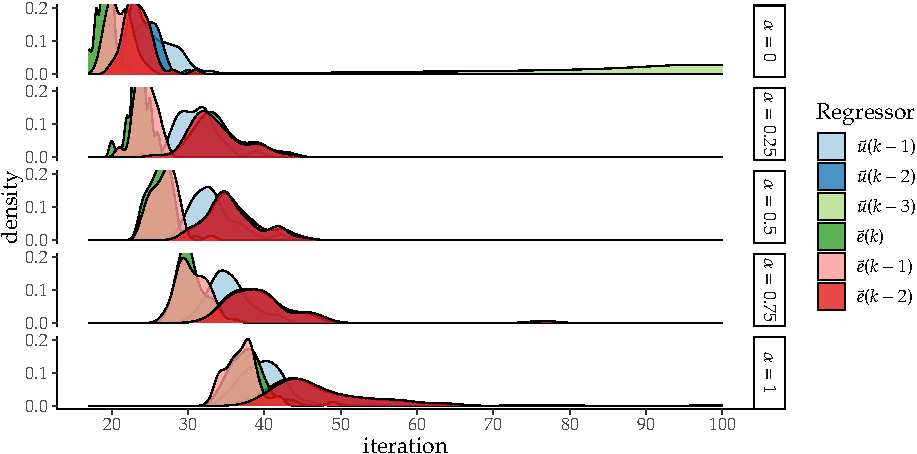
\includegraphics{Figs/Cap5/ex51_iter_con_SEM_ruido.tex.pdf}
  \caption{Probability densities of selection for the regressors selected within 100 iterations considering different values of $\alpha$ for the case without noise.}
  \label{fig:exp51_dens_prob_SR}
\end{figure}
In the figure, it is clear that the method selects the ideal parameters well for all cases. In the case without using the tracking error information, $\alpha=0$, the $\tilde{u}(k-3)$ regressor is chosen with low probability for few iterations but with increasing probability with the increase in iterations.

When tracking error information is taken into account, cases with $\alpha>0$, only the ideal regressors are selected for all 50 realizations. Note that the overall average time to choose the regressors increases with the increase in the $\alpha$ parameter. One possible explanation is that the performance index related to the tracking error, $J_r$, changes little compared to the index related to the prediction error, $J_p$. A probable solution may be to adopt a larger $K$ gain in the calculation of the MSTE (see equation \ref{eq:Jr}).

% As mesmas simulações anteriores são feitas para o caso em que existe ruído de medição (ruído na saída), como no caso B do Exemplo \ref{ex:sis2aord}. A Figura \ref{fig:exp51_ev_rips_a1_CR} mostra a evolução dos RIPs e a Figura \ref{fig:exp51_dens_prob_CR} mostra a densidade de probabilidade de escolha dos regressores em função do número de iterações para cada valor de $\alpha$, considerando esse novo caso.
The same previous simulations are done for the case in which there is measurement noise (noise at the output), as in case B of Example \ref{ex:sis2aord}. Figure \ref{fig:exp51_ev_rips_a1_CR} shows the evolution of RIPs and Figure \ref{fig:exp51_dens_prob_CR} shows the probability density of choice of regressors as a function of the number of iterations for each value of $\alpha$, considering this new case.

  \begin{figure}[htpb]
    \centering
    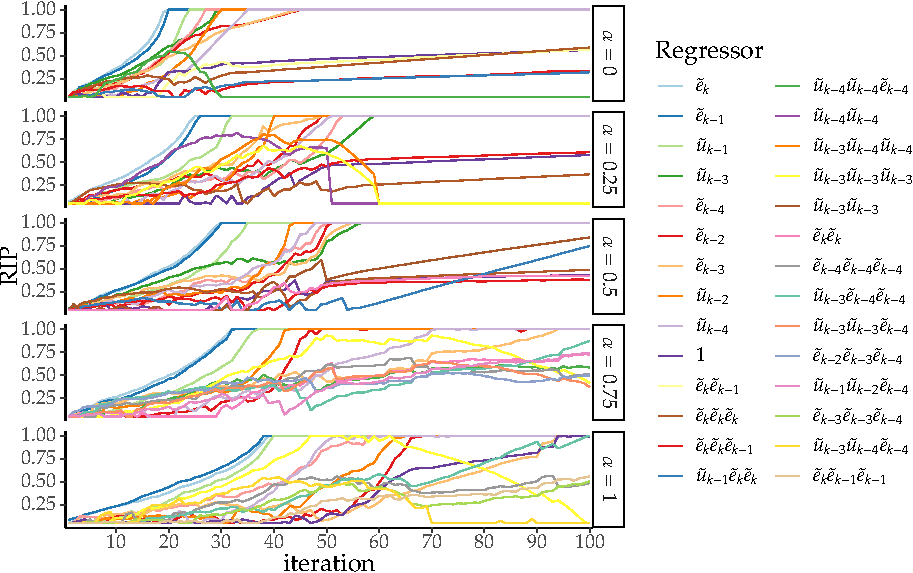
\includegraphics{Figs/Cap5/ex51_rips_evol_CR.tex.pdf}
    \caption{RIPs evolution to different values of parameter $\alpha$ considering data with noise.}
    \label{fig:exp51_ev_rips_a1_CR}
  \end{figure}

    % \footnote{note que são mostrados em cores os RIPs mais relevantes, i.e. aqueles que não convergem para $\mu_{\min}$). Estes outros são mostrados em escala de cinza e não aparecem na legenda por serem muitos (220 regressores). Os repressores ideais são mostrados em linhas mais espessas.}


  \begin{figure}[htpb]
    \centering
    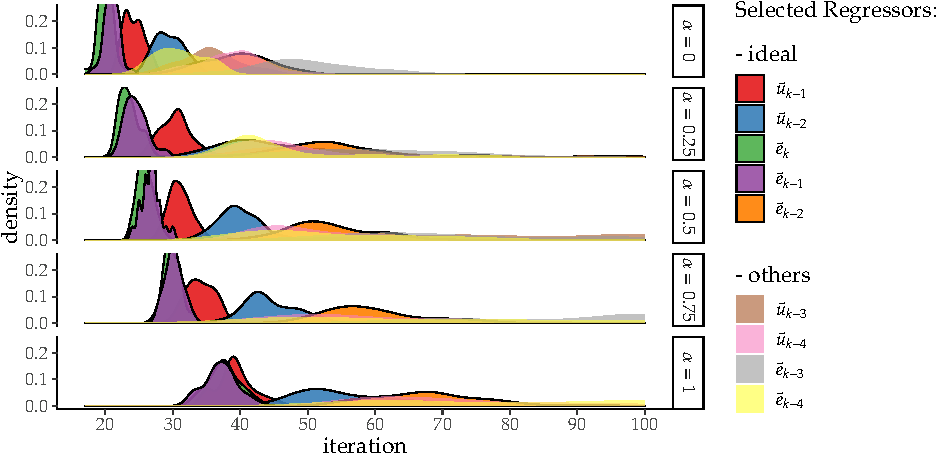
\includegraphics{Figs/Cap5/ex51_iter_con_COM_ruido.tex.pdf}
    \caption{Probability densities of selection for the regressors selected within 100 iterations considering different values of $\alpha$ for the case without noise.}
    \label{fig:exp51_dens_prob_CR}
  \end{figure}

  % Observando a Figura \ref{fig:exp51_ev_rips_a1_CR}, observa-se que os seguintes fatores: 1) em todos os casos os regressores ideais foram selecionados. Com o aumento de $\alpha$ os regressores não ideais têm uma menor densidade de probabilidade de serem escolhidos. Isto fica mais evidente comparando-se várias realizações, como mostra a Figura \ref{fig:exp51_ev_rips_a1_CR}. Comparando $\alpha=0$ com $\alpha>0$ nota-se que a probabilidade de ser selecionar regressores não ideiais diminui para menores iterações. Porém para valores maiores de $\alpha$, nota-se um maior tempo de convergência dos regressores. Por exemplo, nota-se uma quantidade maior de regressores que não convergem para o valor mínimo $\mu_{\min}$ para maiores valores de $\alpha$. O problema da polarização pode ser um dos resposponsáveis por este fator.
  Looking at Figure \ref{fig:exp51_ev_rips_a1_CR}, it is observed the following facts: 1) in all cases the ideal regressors were selected. 2) With the increase of $\alpha$, non-ideal regressors have a lower probability of being chosen. This is more evident when comparing several realizations, as shown in Figure \ref{fig:exp51_dens_prob_CR}. Comparing $\alpha=0$ with $\alpha>0$, it can be seen that the probability of selecting non-ideal regressors decreases for smaller iterations. However, for values greater than $\alpha=0$, there is a longer convergence time for the regressors. For example, we notice a greater number of regressors that do not converge to the minimum value $\mu_{\min}$ for higher values of $\alpha$. The polarization problem may be one of the factors responsible for this behavior.

  % \todo[inline]{    Neste exemplo aplico o ``RaCSS'' ao mesmo sistema de 2a ordem do exemplo anterior, mas agora usando informação do erro de rastreamento no cálculo dos RIPs. \\ Por enquanto estão somente os gráficos, ainda falta análise e algumas tabelas comparativas com ERR.  }

\end{exmp}

